\documentclass[11pt,a4paper]{article}

\usepackage[margin=2.4cm]{geometry}
\usepackage[T1]{fontenc}
\usepackage{lmodern}
\usepackage{microtype}
\usepackage{xcolor}
\usepackage{booktabs}
\usepackage{tabularx}
\usepackage{longtable}
\usepackage{array}
\usepackage{listings}
\usepackage{tikz}
\usetikzlibrary{arrows.meta,positioning,fit,backgrounds}
\usepackage{amsmath}
\usepackage{hyperref}

\definecolor{accent}{HTML}{3B5BDB}
\definecolor{codebg}{HTML}{F5F6F8}
\hypersetup{colorlinks=true,linkcolor=accent,urlcolor=accent}

\lstset{basicstyle=\ttfamily\small, backgroundcolor=\color{codebg}, frame=single, rulecolor=\color{codebg},
  breaklines=true, columns=fullflexible, keepspaces=true, showstringspaces=false, upquote=true,
  xleftmargin=4pt, xrightmargin=4pt, aboveskip=8pt, belowskip=8pt}

% monospace names that may break after / _ . -
\makeatletter
\g@addto@macro\UrlBreaks{\do\_\do\.\do\-}
\makeatother
\urlstyle{tt}
\newcommand{\file}[1]{\nolinkurl{#1}}
\emergencystretch=2.5em
\newcolumntype{L}{>{\raggedright\arraybackslash}X}
\newcolumntype{P}[1]{>{\raggedright\arraybackslash}p{#1}}
\setlength{\parskip}{3pt}

\begin{document}

%--------------------------------------------------------------------- title page
\begin{titlepage}
\centering
\vspace*{3cm}
{\LARGE\bfseries AutoGrader\\[6pt] A Rule-Driven Evaluator for C Programs\par}
\vspace{1cm}
{\large Assignment Report\par}
\vspace{2.5cm}
{\large \textbf{Name:} \rule{6cm}{0.4pt}\par}
\vspace{0.6cm}
{\large \textbf{Roll No.:} \rule{5.4cm}{0.4pt}\par}
\vspace{0.6cm}
{\large \textbf{Course:} \rule{5.6cm}{0.4pt}\par}
\vfill
{\large October 2026\par}
\end{titlepage}

\begin{abstract}
\noindent
This report presents AutoGrader, an agent that grades student C programs without human intervention. Given a
submission and an instructor-written rules file, it compiles and runs the program in a sandbox with fixed time and
memory limits, evaluates nine metrics with independent analyzers (correctness, compiler warnings, structure,
modularity, corner cases, time complexity, memory safety, readability and originality) and combines them into one
weighted grade. For an incorrect program the feedback gives a concrete failing input with the expected output, the
sanitizer diagnosis and an explanation. Readability is judged by an LLM on Groq, and a local Ollama
\texttt{qwen3:4b} model proposes adversarial inputs, explains failures and writes reference solutions so that copying
from an LLM can be detected. Originality is measured on an abstract structural representation of the code that
ignores renaming, formatting and loop style. The system has a Django backend and a plain HTML/CSS frontend and runs on
macOS and Linux. On ten sample submissions, each with a known flaw, the agent detected every flaw, and repeated grading
on both platforms produced identical grades, metric scores and flags.
\end{abstract}

\tableofcontents
\newpage

%=====================================================================
\section{Introduction}
%=====================================================================
When a class submits programs, someone has to run them, decide whether they are correct, how efficient they are and
whether the code is written well. By hand this is slow, inconsistent between graders and does not scale. The task of
this assignment is to build an \emph{intelligent agent} that does the whole job on its own: it takes a C submission and
the instructor's rules, runs the submission safely, checks it against every rule, and returns one overall grade with
feedback that shows the student where the program falls short.

The central requirement is \textbf{reproducibility}: the same submission, judged under the same rules, must receive the
same grade every time the agent runs. This is harder than it sounds, because two of the most useful signals are noisy:
execution time varies with machine load, and LLMs do not always return the same answer. A large part of the design is
about removing that noise without losing the signal.

\subsection{Objectives}
The agent must:
\begin{enumerate}
  \item run the submission safely under fixed time and memory limits and survive programs that crash or never halt;
  \item read the grading rules from a file outside its source code, so rules change without editing the agent;
  \item evaluate each metric with its own analyzer and combine the results using the weights in the rules;
  \item produce feedback that, for an incorrect submission, includes a failing input with the expected output, reports
        memory errors and leaks, and profiles the program;
  \item flag suspected copying from peers, online resources or LLMs;
  \item state the usefulness and limitations of the agent with concrete examples.
\end{enumerate}

\subsection{Summary of the solution}
\begin{longtable}{@{}P{3.8cm}P{11.2cm}@{}}
\toprule
\textbf{Objective} & \textbf{How it is met} \\
\midrule
\endhead
1. Safe execution & Process-group sandbox with CPU-time, memory, output and core-dump limits; hangs, crashes and floods are caught (Section~\ref{sec:sandbox}). \\
2. External rules & JSON rules files, validated on load and in the web editor (Section~\ref{sec:rules}). \\
3. One analyzer per metric & Nine plug-in analyzers, dispatched by a coordinator and combined by weight (Sections~\ref{sec:agent}, \ref{sec:analyzers}). \\
4. Feedback & Failing inputs from hidden tests and generated counter-tests, judged against a reference solution; ASan/UBSan; leak checks; CPU/memory profile; LLM tutor explanations (Section~\ref{sec:feedback}). \\
5. Copy flagging & Abstract structural fingerprints compared against peers and qwen3-generated solutions (Section~\ref{sec:similarity}). \\
6. Usefulness \& limitations & Four of each with concrete cases, included in every report (Section~\ref{sec:ul}). \\
Reproducibility & Seeded generation, deterministic ordering, content-addressed LLM cache, CPU-time limits; verified experimentally on macOS and Linux (Section~\ref{sec:repro}). \\
\bottomrule
\end{longtable}

%=====================================================================
\section{System design}
%=====================================================================
\subsection{Architecture}
The system has two parts. The \textbf{engine} (\file{engine/}) is a framework-independent Python package containing the
agent; it can be used from the command line. The \textbf{web application} (\file{grader/}, Django) stores submissions,
queues them for a background worker and renders reports. Figure~\ref{fig:pipeline} shows the agent's pipeline.

\begin{figure}[h]
\centering
\resizebox{\textwidth}{!}{%
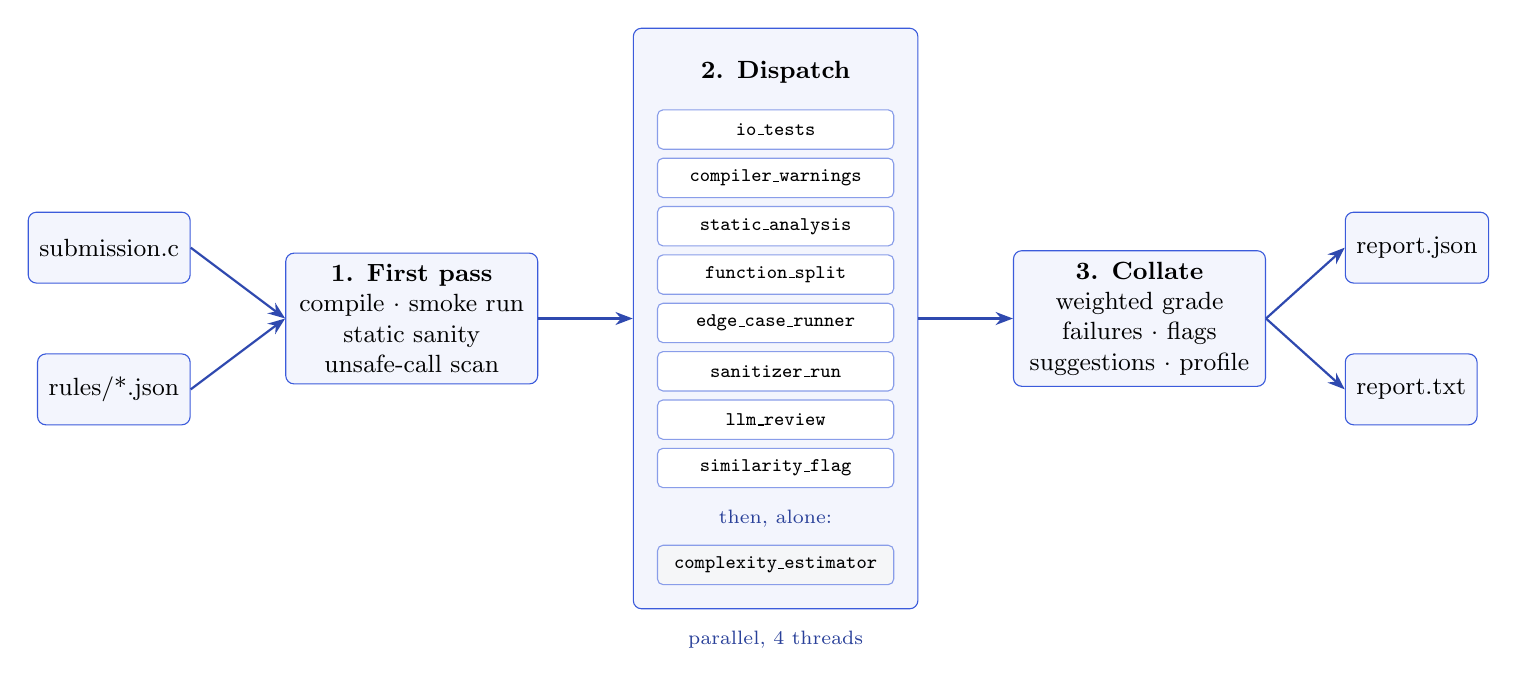
\begin{tikzpicture}[
  box/.style={draw=accent, rounded corners=3pt, fill=accent!6, align=center, font=\small, minimum height=9mm, inner sep=4pt},
  an/.style={draw=accent!60, rounded corners=2pt, fill=white, font=\scriptsize\ttfamily, minimum width=30mm, minimum height=5mm, inner sep=1.5pt},
  arr/.style={-{Stealth[length=2.2mm]}, thick, accent!80!black}]
  \node[font=\small\bfseries] (dt) at (0,0) {2. Dispatch};
  \node[an, below=2mm of dt] (a1) {io\_tests};
  \node[an, below=1mm of a1] (a2) {compiler\_warnings};
  \node[an, below=1mm of a2] (a3) {static\_analysis};
  \node[an, below=1mm of a3] (a4) {function\_split};
  \node[an, below=1mm of a4] (a5) {edge\_case\_runner};
  \node[an, below=1mm of a5] (a6) {sanitizer\_run};
  \node[an, below=1mm of a6] (a7) {llm\_review};
  \node[an, below=1mm of a7] (a8) {similarity\_flag};
  \node[font=\scriptsize, text=accent!70!black, below=1.5mm of a8] (sep) {then, alone:};
  \node[an, below=1mm of sep, fill=codebg] (a9) {complexity\_estimator};
  \begin{scope}[on background layer]
    \node[draw=accent, rounded corners=3pt, fill=accent!6, inner sep=3mm, fit=(dt)(a1)(a9)] (disp) {};
  \end{scope}
  \node[font=\scriptsize, text=accent!70!black, below=1.5mm of disp] {parallel, 4 threads};
  \node[box, left=12mm of disp, minimum width=32mm] (fp) {\textbf{1. First pass}\\compile $\cdot$ smoke run\\static sanity\\unsafe-call scan};
  \node[box, left=12mm of fp, yshift=9mm] (sub) {submission.c};
  \node[box, left=12mm of fp, yshift=-9mm] (rules) {rules/*.json};
  \node[box, right=12mm of disp, minimum width=32mm] (col) {\textbf{3. Collate}\\weighted grade\\failures $\cdot$ flags\\suggestions $\cdot$ profile};
  \node[box, right=10mm of col, yshift=9mm] (json) {report.json};
  \node[box, right=10mm of col, yshift=-9mm] (txt) {report.txt};
  \draw[arr] (sub.east) -- (fp.west);
  \draw[arr] (rules.east) -- (fp.west);
  \draw[arr] (fp) -- (disp);
  \draw[arr] (disp) -- (col);
  \draw[arr] (col.east) -- (json.west);
  \draw[arr] (col.east) -- (txt.west);
\end{tikzpicture}}
\caption{The agent's pipeline (\file{engine/agent.py}).}
\label{fig:pipeline}
\end{figure}

\subsection{Tools}
\noindent\begin{tabularx}{\textwidth}{@{}P{4.6cm}L@{}}
\toprule
\textbf{Tool} & \textbf{Used for} \\
\midrule
clang / gcc & Compilation, warnings, \texttt{-fsanitize=address,undefined} \\
AddressSanitizer, UBSan & Buffer overflows, use-after-free, undefined behaviour (e.g. signed overflow) \\
macOS \texttt{leaks}, LeakSanitizer, valgrind & Memory-leak detection with the leaking source line \\
lizard & Cyclomatic complexity and length per function \\
Groq (\texttt{openai/gpt-oss-120b}) & Readability judgement \\
Ollama (\texttt{qwen3:4b}, local) & Adversarial test inputs, tutor explanations, AI-written reference solutions \\
Django + SQLite & Web backend, submission history, background worker \\
HTML / CSS & Frontend (one hand-written stylesheet, light and dark) \\
\bottomrule
\end{tabularx}

\subsection{The rules file}\label{sec:rules}
Rules are JSON files in \file{rules/}. Everything that defines a grading run is in the file: limits, compile flags,
the input format, the reference solution, and the list of metrics, each with an analyzer name, a weight and parameters.
The file \file{rules/add_two_integers.json} reproduces the assignment's example and adds the information the agent
needs to generate its own tests:

\begin{lstlisting}
"reference_solution": "problems/add_two_integers/reference.c",
"input_format": {"lines": [[{"name": "a", "type": "int"}, {"name": "b", "type": "int"}]]},
"metrics": [
  {"name": "correctness", "analyzer": "io_tests", "weight": 0.20, "params": {"testset_dir": "tests/add/"}},
  {"name": "logical", "analyzer": "edge_case_runner", "weight": 0.10,
   "params": {"cases": ["negatives", "zero", "int_overflow", "whitespace", "llm"]}},
  ...
]
\end{lstlisting}

The \texttt{input\_format} describes stdin as lines of typed fields (\texttt{int}, \texttt{long}, \texttt{uint},
\texttt{float}, \texttt{word}) with optional ranges; a field can repeat as many times as another field's value, which
describes arrays. The rules are validated on load: an unknown analyzer, a duplicate metric, a negative weight or
malformed JSON is rejected with a clear message, also in the web editor. Weights that do not sum to 1 are normalised
and the report notes it. A second rules file, \file{rules/sum_array.json}, defines a harder problem (sum of up to
$10^6$ integers, required $O(n)$), so that complexity, leak and copy detection have something real to detect.

%=====================================================================
\section{Methodology}
%=====================================================================
\subsection{Safe execution}\label{sec:sandbox}
Every run of student code goes through \file{engine/sandbox.py}:
\begin{itemize}
  \item \textbf{Time limit on CPU time.} The limit counts user + system CPU time, as on competitive-programming judges.
        \texttt{RLIMIT\_CPU} kills spinning programs, and a wall-clock backstop of $3\times$ the limit plus 1\,s kills
        programs that hang without using CPU. The program runs in its own process group, which is killed as a whole.
  \item \textbf{Memory limit on resident memory.} The parent polls the program's memory every 2--10\,ms
        (\texttt{libproc} on macOS, \file{/proc/<pid>/status} on Linux) and kills it above the cap; the peak from
        \texttt{wait4} is checked afterwards. On Linux, \texttt{RLIMIT\_AS} at twice the limit is a safety net.
  \item \textbf{Output limit} (\texttt{RLIMIT\_FSIZE}), no core dumps, a private working directory and a minimal environment.
  \item \textbf{Files instead of pipes} for stdin and stdout, so a program printing in an endless loop cannot deadlock the grader.
  \item \textbf{No dangerous calls.} Programs calling \texttt{system}, \texttt{fork}, \texttt{exec*}, \texttt{popen},
        \texttt{socket}, \texttt{kill}, \texttt{unlink} and similar are never executed.
\end{itemize}

\subsection{The coordinator}\label{sec:agent}
The coordinator (\file{engine/agent.py}) works in three phases.

\textbf{First pass.} A cheap sanity sweep: compile with \texttt{-O2 -Wall -Wextra -std=c11}, run the sample input under
the limits, and check that \texttt{main} exists, input is read and output is written. If the smoke run times out, the
report gets a \texttt{suspected\_infinite\_loop} flag; the execution-based analyzers (correctness, logic, complexity,
memory safety) are skipped with score 0, the source-only analyzers still run, and a partial report is produced.
A compile error or a dangerous call has the same effect.

\textbf{Dispatch.} Each metric is sent to its analyzer, in parallel on four threads. The complexity analyzer is
timing-sensitive, so it runs alone afterwards. An exception in an analyzer becomes a score of 0 with the error recorded;
it cannot break the report.

\textbf{Collation.} With normalised weights $w_i$ and analyzer scores $s_i\in[0,1]$:
\[ \text{grade} = 100 \cdot \sum_i w_i\, s_i . \]
Results are combined in the order of the rules file, never in completion order. Failures from all analyzers are merged
and de-duplicated, suggestions are ranked by the points their metric lost, and a profile is assembled.

\subsection{The analyzers}\label{sec:analyzers}
\begin{longtable}{@{}P{3.3cm}P{7.6cm}P{3.9cm}@{}}
\toprule
\textbf{Metric (analyzer)} & \textbf{Method} & \textbf{Score} \\
\midrule
\endhead
correctness (\file{io_tests}) & Runs every hidden test, compares the output (whitespace-insensitive by default), records verdict, CPU time and peak memory per test. & passed / total \\
syntax (\file{compiler_warnings}) & Compiles with the rule's flags, counting warnings individually even under \texttt{-Werror}. & $1-0.1\times$warnings; 0 on errors \\
structure (\file{static_analysis}) & lizard cyclomatic complexity and function length against the limits; comments, header comment, single-block code, globals, \texttt{goto}, long lines, magic numbers. & $1-\sum$ deductions \\
modularity (\file{function_split}) & Number of functions, helpers besides \texttt{main}, share of code in \texttt{main}, unused helpers. & 1 if enough functions; 0.3 if only \texttt{main} \\
logical (\file{edge_case_runner}) & Generated corner cases and LLM counter-tests judged against the reference solution (Section~\ref{sec:counter}). & passed / total \\
complexity (\file{complexity_estimator}) & Timing curve plus static loop analysis (Section~\ref{sec:complexity}). & 1 if within bound, $-0.5$ per class above \\
memory\_safety (\file{sanitizer_run}) & ASan + UBSan on every hidden test; leak check (Section~\ref{sec:memory}). & $1-0.25\times$distinct issues \\
readability (\file{llm_review}) & Groq LLM with a fixed rubric (Section~\ref{sec:readability}). & LLM score / 10 \\
originality (\file{similarity_flag}) & Abstract structural similarity (Section~\ref{sec:similarity}). & 1 below threshold; flagged above \\
\bottomrule
\end{longtable}

\subsection{Counter-test generation}\label{sec:counter}
The assignment asks the agent to generate counter test cases covering corner cases. The edge-case analyzer builds
inputs from the rules' \texttt{input\_format} in categories:

\noindent\begin{tabularx}{\textwidth}{@{}P{3.2cm}L@{}}
\toprule
\texttt{zero} & all zero; zero mixed with other values; minimum size \\
\texttt{negatives} & $-1$, small and large negative values \\
\texttt{int\_overflow} & $[\max]$, $[\min]$, $[\max, 1]$, $[\min, -1]$, $[\max, \min]$ for full-range integers \\
\texttt{boundaries} & every field at its declared minimum and maximum \\
\texttt{whitespace} & the same data with tabs, extra spaces, blank lines, no trailing newline \\
\texttt{large}, \texttt{single}, \texttt{empty} & maximum size, $n=1$, $n=0$ \\
\texttt{llm} & qwen3 reads the problem \emph{and the student's code} and proposes inputs likely to break this program \\
\bottomrule
\end{tabularx}

\medskip
The random generator for each category is seeded from a hash of the rules, so every run produces the same inputs.
Every LLM-proposed input is validated against the input format before use; this was necessary because qwen3 often
proposed, for example, a single number where two integers were required (2 of 5 proposals were rejected for
\file{add.c}). Expected outputs come from the compiled reference solution, which acts as an oracle.

\subsection{Complexity estimation}\label{sec:complexity}
For each input size $n$ in the rules, an input of exactly that size is generated, the program runs three times, and the
\emph{minimum} CPU time is kept, as the estimator least affected by noise. With the smallest size as a baseline, the
slope of $\log(t_n - t_0)$ against $\log n$ is fitted, ignoring points below a 4\,ms noise floor. Slope bands map to
classes: below 0.35 is $O(1)$ or $O(\log n)$, below 1.35 is $O(n)$ or $O(n\log n)$, below 2.4 is $O(n^2)$, and above
that $O(n^3)$. A static estimate (maximum loop nesting depth, recursion, use of \texttt{qsort}) breaks ties and is used
when the timings are flat. A timeout at some size means the required bound is exceeded.

\subsection{Memory analysis and profiling}\label{sec:memory}
The program is rebuilt with \texttt{-fsanitize=address,undefined -g} and run on every hidden test. Diagnostics are
parsed into distinct \emph{(kind, source line)} issues: heap, stack and global buffer overflows, use-after-free, double
free and undefined behaviour. The source line is taken from the first stack frame inside the student's file. Leaks are
detected by macOS \texttt{leaks} on macOS, and by LeakSanitizer (or valgrind, if installed) on Linux; all three report
the leaking line. The profile lists the maximum CPU time, wall time and peak memory over the hidden tests, plus the
scaling curve from the complexity analyzer.

\subsection{Readability with an LLM}\label{sec:readability}
The code is sent to Groq with line numbers and a fixed 0--10 rubric covering names, comments, formatting, consistency
and clarity; correctness is explicitly excluded. The request uses temperature 0, seed 42 and JSON output, and the
answer provides the score, the reasons and line-specific suggestions.

The assignment's example uses \texttt{llama-3.3-70b-versatile}, but that model is no longer available on Groq for this account (HTTP 404, \texttt{model\_not\_found}). The available
models were compared on \file{add.c}: \texttt{openai/gpt-oss-120b} gave 5/10 with accurate suggestions;
\texttt{qwen/qwen3.8-27b} also gave 5/10 but claimed a missing space that was not missing. \texttt{openai/gpt-oss-120b}
was chosen; it gives exactly the 5/10 that the assignment's example shows for this program.

\subsection{Originality: abstract structural similarity}\label{sec:similarity}
Comparing raw text is defeated by renaming variables or reformatting. AutoGrader compares programs on an abstract
representation instead:
\begin{enumerate}
  \item \textbf{Canonicalise:} \texttt{for (A; B; C) S} becomes \texttt{A; while (B) \{ S C; \}}; braces are dropped,
        so optional braces do not matter; comments and whitespace are removed.
  \item \textbf{Abstract:} identifiers become \texttt{V}; literals become \texttt{N}, \texttt{S} or \texttt{C};
        integer types become \texttt{INT}; all loops become \texttt{LOOP}; \texttt{++}/\texttt{--} become \texttt{INC};
        compound assignments become \texttt{OPEQ}. Library calls are kept, because they carry meaning.
  \item \textbf{Compare} two views: token 5-grams (Jaccard similarity $J$) and the control-flow skeleton of loops,
        branches, returns and library calls (sequence alignment ratio $S$); similarity $= 0.75J + 0.25S$.
  \item \textbf{Exclude base code:} 5-grams that also occur in the instructor's reference solution are removed first,
        so shared boilerplate is not evidence (as in MOSS).
  \item \textbf{Corpus:} all peer submissions of the problem, plus three solutions written by qwen3 for the same
        problem statement, so copying from an LLM is detected the same way as copying from a peer.
  \item \textbf{Size gate:} programs shorter than 50 abstract tokens are not flagged, because short programs such as a
        six-line $a+b$ are written identically by almost everyone.
\end{enumerate}
A submission whose similarity reaches the threshold (0.85) is flagged as \texttt{suspected\_copy} or
\texttt{suspected\_llm\_copy} for human review, and its originality score falls linearly to 0 at similarity 1.

\subsection{Feedback generation}\label{sec:feedback}
Each failure is reported with the input, the expected output and the actual output, followed by three explanations:
the \textbf{sanitizer} diagnosis from re-running that input under ASan/UBSan; a deterministic \textbf{WHY} (for
example, detecting that the expected value lies outside the 32-bit range and the program's output differs from it by
exactly $2^{32}$, which means the value wrapped around); and an \textbf{AI tutor} note from qwen3 giving the root cause
and the fix. Suggestions are ranked by how many points their metric lost. Each grading writes a JSON report for
machines and a text report for the student.

\paragraph{Running qwen3 reliably.} The installed \texttt{qwen3:4b} kept producing long reasoning text even with
thinking disabled; one code-generation request took 70\,s and returned no code. Requesting grammar-constrained JSON
output (Ollama's JSON mode) makes it answer directly in about 4\,s. Code is requested as an array of lines, because
escaping a whole program into one JSON string triggered Ollama's repeat limit.

%=====================================================================
\section{Reproducibility}\label{sec:repro}
%=====================================================================
The following mechanisms make the grade a function of the submission and the rules only:
\begin{itemize}
  \item \textbf{Seeded inputs:} all generated inputs come from random generators seeded with a hash of the rules.
  \item \textbf{Deterministic order:} results are combined in rules order; all file and corpus listings are sorted.
  \item \textbf{LLM cache:} every LLM request is keyed by a hash of provider, model, messages, temperature and seed. The
        first answer is stored and replayed on every later run, and the cache is consulted before checking whether the
        service is reachable. Deterministic model failures are cached too, so a later successful retry cannot change a grade.
  \item \textbf{CPU-time limits} and minimum-of-$N$ timing mapped onto discrete complexity classes; the web worker grades
        one submission at a time.
  \item \textbf{Audit trail:} each report stores hashes of the submission, the rules, and the rules + tests + reference
        solution, plus the corpus hash and tool versions.
\end{itemize}

\subsection{Two noise sources found during testing}
\paragraph{The LLM is not deterministic.} Three fresh Groq requests with temperature 0 and seed 42 scored
\file{sum_leak.c} 7, 8 and 7 out of 10. Without the cache, the overall grade would vary by 0.5 points between runs.
The cache is therefore essential, not an optimisation.

\paragraph{Wall-clock time is not reliable.} The first launch of a freshly compiled binary took 0.42\,s of wall-clock
time for 0.01\,s of CPU time, because macOS scans new binaries. Under load, this once pushed the correct \file{add.c}
past the 1\,s limit, and it was flagged as an infinite loop and graded 40 instead of 75.72. Measuring the time limit in
CPU time removed the problem.

%=====================================================================
\section{Implementation}
%=====================================================================
\begin{itemize}
  \item \textbf{Web UI} (\file{grader/}): upload one or several \texttt{.c} files or paste code; a report page with the
        grade, a per-metric table with evidence, failure cards, suggestions, profile, the source code with flagged lines
        highlighted, and the usefulness and limitations section; submission history with statistics and a ``clear all''
        button; a rules editor with validation.
  \item \textbf{Unattended use:} \texttt{python -m engine <files> --rules <rules>} or
        \texttt{manage.py grade} for batches, and an HTTP API (\texttt{POST /api/grade/}).
  \item \textbf{Cross-platform:} tested on macOS (Apple clang 21) and, in containers installed by the setup script, on
        Ubuntu 22.04 (Python 3.10, gcc 11), Debian 12 (Python 3.11, gcc 12), Ubuntu 24.04 (gcc 13) and Fedora 41 (gcc 14),
        plus x86\_64 Ubuntu under emulation. Python 3.10 or newer is required. Running the code there exposed three problems, all fixed: memory peaks inherited from the grader process (solved with a small C launcher, \file{engine/launcher.c}); sanitizer reports without line numbers under gcc (solved with a shared parser); and cached LLM answers being ignored when Ollama was unreachable (solved by consulting the cache first). A setup script and Docker files handle installation. Testing on emulated x86\_64 exposed one
        more problem: AddressSanitizer cannot run there, and the analyzer reported a false 10/10 for memory safety. The
        agent now self-tests the sanitizers first and, if they do not work, leaves the metric out of the grade with a flag
        instead of trusting silence.
\end{itemize}

%=====================================================================
\section{Results}
%=====================================================================
\subsection{The assignment's worked example}
Table~\ref{tab:example} compares the agent's result for the assignment's \file{add.c} with the example in the
assignment.

\begin{table}[htbp]
\centering
\small
\begin{tabular}{@{}lrrp{7.6cm}@{}}
\toprule
\textbf{Metric} & \textbf{Example} & \textbf{AutoGrader} & \textbf{Reason for any difference} \\
\midrule
correctness & 18/20 & 16/20 & 8 of 10 tests pass in both; the example's 18/20 does not match its own ``8 of 10'', the agent scores passed/total \\
syntax & 9/10 & 10/10 & clang and gcc report no warning for this file; the example's \texttt{-Wunused-parameter} cannot occur, as \texttt{main} has no parameters \\
structure & 6/10 & 7/10 & no comments ($-0.2$) and a single block ($-0.1$) \\
modularity & 3/10 & 3/10 & only \texttt{main} \\
logical & 8/10 & 7.2/10 & 13 of 18 corner cases; fails 4 of 5 overflow cases and 1 of 3 qwen3 cases \\
complexity & 10/10 & 10/10 & $O(1)$ confirmed \\
memory\_safety & 10/10 & 7.5/10 & UBSan reports signed overflow at line 5 on hidden test 07: undefined behaviour is a real memory-safety finding \\
readability & 5/10 & 5/10 & single-letter names, no comments \\
originality & 10/10 & 10/10 & too short to judge; not flagged \\
\midrule
\textbf{grade} & \textbf{89} & \textbf{75.72} & \\
\bottomrule
\end{tabular}
\caption{The assignment's example versus the agent's result for \file{add.c}.}
\label{tab:example}
\end{table}

The failing case is reported as the assignment requires, with the expected output beside it:

\noindent\begin{minipage}{\linewidth}
\begin{lstlisting}[basicstyle=\ttfamily\footnotesize]
Test 07  (correctness, WA)
   INPUT:     2147483647 1
   EXPECTED:  2147483648
   GOT:       -2147483648  [exit 0]
   SANITIZER: runtime error at line 5: signed integer overflow: 2147483647 + 1
              cannot be represented in type 'int'
   WHY:       The correct result does not fit in a 32-bit int, so the computation
              wrapped around (signed integer overflow is undefined behaviour in C).
              Use a wider type such as long long for the result.
   AI TUTOR:  The sum of 2147483647 and 1 exceeds the maximum value for a 32-bit
              signed integer, causing an overflow. Fix: Use a 64-bit integer type
              for the sum.
\end{lstlisting}
\end{minipage}

\subsection{All sample submissions}
Ten sample submissions were prepared, each with a known flaw (or none), to check that every metric detects what it
should. Table~\ref{tab:samples} shows the results on macOS.

\begin{longtable}{@{}P{3.7cm}P{4.0cm}rP{5.6cm}@{}}
\caption{Results on the sample submissions.}\label{tab:samples}\\
\toprule
\textbf{Submission} & \textbf{Planted flaw} & \textbf{Grade} & \textbf{Detected} \\
\midrule
\endhead
\file{add.c} & assignment example: \texttt{int} sum & 75.72 & overflow on 2 hidden tests and 4 corner cases; UB at line 5; only \texttt{main} \\
\file{add_clean.c} & none & 100.00 & nothing to report \\
\file{add_infinite.c} & waits for a \texttt{.} that never arrives & 40.00 & \texttt{suspected\_infinite\_loop}; partial report \\
\file{add_syntax_error.c} & missing \texttt{;} & 26.00 & \texttt{compile\_failed} with the line; source metrics still graded \\
\file{sum_good.c} & none (but copied by \file{sum_copy.c}) & 89.50 & \texttt{suspected\_copy}, similarity 1.00 \\
\file{sum_copy.c} & renamed, \texttt{for}$\rightarrow$\texttt{while}, restyled copy & 88.00 & \texttt{suspected\_copy}, similarity 1.00 \\
\file{sum_ai.c} & qwen3's solution, renamed and re-commented & 85.50 & \texttt{suspected\_llm\_copy}, similarity 1.00 \\
\file{sum_quadratic.c} & correct but $O(n^2)$ & 79.50 & slope 1.88 $\Rightarrow O(n^2)$; time limit at $n=320\,000$ \\
\file{sum_leak.c} & \texttt{int} accumulator; \texttt{malloc} never freed & 77.55 & 5/8 tests; leak at line 12; UB at line 14 \\
\file{sum_fixed_buffer.c} & \texttt{int buf[100]}, any $n$ & 82.64 & 6/8 tests; stack-buffer-overflow at line 6 \\
\bottomrule
\end{longtable}

Every planted flaw was detected by the metric meant to detect it, and the flawless \file{add_clean.c} scored 100.
The complexity curve separates the algorithms clearly: \file{sum_good.c} took 3.4, 6.7 and 20.4\,ms at
$n = 20\,000$, $80\,000$ and $320\,000$ (slope 0.65, $O(n)$), while \file{sum_quadratic.c} went from 11.6 to 156\,ms
between the first two sizes (slope 1.88) and exceeded the limit at the third.

\subsection{Copy detection}
\file{sum_copy.c} renames every identifier of \file{sum_good.c}, replaces the \texttt{for} loop with a \texttt{while}
loop, changes brace style and rewrites the comments; \file{sum_ai.c} does the same to qwen3's solution. Both reduce to
exactly the same abstract stream as their source and are flagged at similarity 1.00. Before \texttt{for}/\texttt{while}
canonicalisation and brace removal were added, the first pair scored only 0.57 and was missed. Independent solutions
stayed well below the threshold: the highest similarity of \file{sum_quadratic.c} to any other program was 0.47.

An observation from the AI corpus: the three qwen3 solutions (seeds 1--3, temperature 0.7) differ as text but are
structurally identical. A single generated solution would detect the same copies; more diverse references would need
different prompts or models.

\subsection{Reproducibility experiments}
\texttt{scripts/check\_reproducibility.py} grades every sample several times and compares the grade, every metric score
and the set of flags.

\noindent\begin{tabularx}{\textwidth}{@{}P{5.4cm}P{3.2cm}L@{}}
\toprule
\textbf{Experiment} & \textbf{Platform} & \textbf{Result} \\
\midrule
9 samples $\times$ 3 runs, Groq enabled & macOS & identical \\
9 samples $\times$ 3 runs & Ubuntu 24.04 (gcc 13) & identical \\
both of the above at the same time (heavy load) & macOS + Linux & identical on both \\
\file{sum_ai.c} $\times$ 2 runs & macOS & identical (85.50) \\
web UI and HTTP API vs command line & macOS, Linux & identical (75.72 for \file{add.c}) \\
10 samples $\times$ 2 runs each on Ubuntu 22.04 and Debian 12 & Python 3.10 / 3.11, gcc 11 / 12 & identical; same grades as Ubuntu 24.04 \\
\bottomrule
\end{tabularx}

\medskip
Across platforms, 8 of 9 samples received exactly the same grade on Linux as on macOS. \file{sum_quadratic.c} scored
78.90 on Linux and 79.50 on macOS: its $O(n^2)$ algorithm is close to the time limit on a 2-CPU virtual machine. This
is expected, because time limits are a property of the machine; each machine is reproducible on its own.

%=====================================================================
\section{Usefulness and limitations}\label{sec:ul}
%=====================================================================
\subsection{Usefulness}
\begin{enumerate}
  \item \textbf{Large programming courses.} A 300-student lab is graded with one command. Every student is judged by the
        same rubric and receives the exact failing input (\texttt{2147483647 1}, expected \texttt{2147483648}) instead of a
        bare mark.
  \item \textbf{Coding-interview screening.} For ``sum an array in $O(n)$'', a nested-loop solution is separated by the
        timing curve (\file{sum_quadratic.c} exceeds the limit at $n = 320\,000$) and an \texttt{int} accumulator by the
        overflow corner cases. Every rejection can be justified metric by metric.
  \item \textbf{Plagiarism and LLM-copy triage.} Renamed and restyled copies of a peer (\file{sum_copy.c}) or of an LLM
        (\file{sum_ai.c}) are flagged at 1.00, so instructors review only the flagged submissions.
  \item \textbf{Self-paced practice.} At any hour a student receives \emph{memory leak at line 12}, a sanitizer trace and
        an explanation of the root cause, without staff time.
\end{enumerate}

\subsection{Limitations}
Each limitation names a concrete case where the agent's verdict is wrong or unreliable.
\begin{enumerate}
  \item \textbf{Tests cannot prove correctness.} A program that recognises the hidden inputs and prints their stored
        answers, or one that fails only for $n = 99\,991$, receives full correctness marks.
  \item \textbf{Timing-based complexity is unreliable for small inputs.} With sizes $[1, 10, 100]$, an $O(n^2)$ program runs
        in under 1\,ms at every size. The static fallback then counts \texttt{for (i = 0; i < 3; i++)} as an $O(n)$ loop and
        treats a recursive merge sort (two self-calls) as possibly exponential.
  \item \textbf{Similarity cannot judge short programs and misses semantic rewrites.} A copied six-line $a+b$ receives
        full originality marks because of the size gate, and a copy rewritten from a loop into recursion is not flagged.
  \item \textbf{Verdicts depend on the compiler and the machine.} \texttt{while (b != 0) \{ s += 1; \}} never terminates,
        but clang \texttt{-O2} may delete this side-effect-free loop (C11 \S6.8.5p6). We observed this: the program finished
        in 6\,ms, and the agent reported a wrong answer instead of an infinite loop. Likewise, \file{sum_fixed_buffer.c}
        crashes for $n = 20\,000$ on Linux but not on macOS, because the default stack sizes differ.
\end{enumerate}
A further caveat concerns readability: the cache makes re-grading identical, but clearing it or changing the model, as was forced when \texttt{llama-3.3-70b-versatile} became unavailable, can change the readability score for the same code.

%=====================================================================
\section{Challenges and lessons learned}
%=====================================================================
\begin{itemize}
  \item \textbf{Platform differences are invisible until tested.} macOS ignores \texttt{RLIMIT\_AS}; LeakSanitizer does
        not exist there; and on Linux the memory peak of the grader leaked into the student program's statistics, making
        every test fail once the grader grew past 64\,MB. Each was found only by running the code on the platform.
  \item \textbf{``Deterministic'' LLM settings are not deterministic.} Temperature 0 with a fixed seed still varied
        between 7 and 8 out of 10. Reproducibility had to come from caching, not from model settings.
  \item \textbf{Small models need constraints.} qwen3 produced unusable output until JSON mode was forced, and its
        proposed inputs had to be validated against the input format.
  \item \textbf{Similarity needs domain knowledge.} Without canonicalising loops and braces a disguised copy was missed;
        without the size gate the assignment's own \file{add.c} was flagged as an LLM copy.
\end{itemize}

%=====================================================================
\section{Conclusion and future work}
%=====================================================================
AutoGrader meets all six objectives of the assignment. It runs untrusted C code safely, reads all grading decisions from
an external rules file, evaluates nine metrics with independent analyzers, explains each failure with a concrete input,
the expected output, a sanitizer diagnosis and a tutor note, flags copies of peers and of LLM output, and documents its
own usefulness and limitations. Above all, it keeps the contract: repeated grading of every sample produced identical
results on macOS and on Linux, including under heavy load.

Possible extensions are: property-based shrinking of failing inputs to the smallest counterexample; mutation testing of
the hidden test set to measure how many bugs it can catch; container-level isolation (seccomp, no network) for
high-stakes use; and calibrating time limits to the grading machine automatically by timing the reference solution.

\appendix
%=====================================================================
\section{Running the agent}
%=====================================================================
\begin{lstlisting}
# setup (macOS)
python3 -m venv .venv && .venv/bin/pip install -r requirements.txt
echo 'GROQ_API_KEY=...' > .env && ollama pull qwen3:4b
.venv/bin/python manage.py migrate

# setup (Linux)
./scripts/setup_linux.sh        # or: docker compose up --build

# web UI
.venv/bin/python manage.py runserver 8000

# unattended grading
.venv/bin/python -m engine submissions/add_two_integers/add.c --rules rules/add_two_integers.json
.venv/bin/python manage.py grade submissions/sum_array/*.c --rules rules/sum_array.json --save

# HTTP API
curl -F file=@add.c -F rules=add_two_integers.json http://localhost:8000/api/grade/

# reproducibility check
.venv/bin/python scripts/check_reproducibility.py --runs 3
\end{lstlisting}

%=====================================================================
\section{Project structure}
%=====================================================================
\begin{lstlisting}[basicstyle=\ttfamily\footnotesize]
engine/           agent.py (coordinator), sandbox.py, launcher.c, context.py, inputs.py,
                  clexer.py, sanitizers.py, llm.py, explain.py, report.py, analyzers/
grader/           Django app: models, services (worker), views, templates, static CSS
rules/            add_two_integers.json, sum_array.json
problems/         statements and reference solutions
tests/            hidden tests (NN.in / NN.out)
submissions/      sample submissions; web uploads in submissions/<problem>/uploads/
corpus/           qwen3-generated reference solutions
reports/          generated JSON and text reports
scripts/          check_reproducibility.py, setup_linux.sh
docs/             this report and the detailed design document
\end{lstlisting}

\end{document}
